% Roteiro Fisica Experimental I
%**********************************

% Configuração General

\documentclass[12pt,a4paper,]{book}
%\documentclass[oneside]{book}
%\documentclass[12pt,a4paper,draft]{book}
%\documentclass[12pt,draft]{report}
%\documentclass[12pt]{report}

% Options possibles : 10pt, 11pt, 12pt (tamanho da fonte)
%   oneside, twoside (recto simple, recto-verso)
%   draft, final (estado de desenvolvimento)

\usepackage[portuguese]{babel} 

%\usepackage[latin1]{inputenc} % LaTeX, comprends les accents !
%\usepackage[applemac]{inputenc}
% margins 
\usepackage[margin=2.cm,top=2.cm]{geometry} 
%\usepackage[showframe]{geometry}
\usepackage{textpos}


\textwidth 16.7cm
\textheight 23.5cm
%\oddsidemargin 1.0cm
%\setlength{\hoffset}{-0.7cm}
%\evensidema	rgin 0.9cm
%\topmargin 7.5cm
%\topmargin -1.5cm
\parindent 0cm
\parskip 0.5cm
%
%\input epsf.tex
\usepackage[pdftex]{graphicx}
\usepackage[font=small,labelfont=sl]{caption}
%links
\usepackage{hyperref}
%\usepackage[dvips]{graphicx}
%\usepackage{pslatex}
%\usepackage{epsfig}
\usepackage{array}
\usepackage{fancyheadings}
\setlength{\headheight}{25pt} 
%\usepackage[spanish]{babel}
%\usepackage[latin1]{inputenc}
\usepackage{palatino}
\usepackage{mathtools}
%\usepackage{amsmath}
\usepackage{color}
 \definecolor{gray}{RGB}{128,128,128}
%
\usepackage{subfigure} 
\usepackage{enumerate}
\usepackage{mathabx}
\usepackage{multirow}
\usepackage{array}
\usepackage{verbatim}
\renewcommand{\arraystretch}{1.5}
%
\usepackage{hyperref}
%
\usepackage{setspace}
\singlespacing
\usepackage{titlesec}
\titlespacing{\section}{0pt}{0.5cm}{-0.2cm}
%\onehalfspacing
%\doublespacing
%\setstretch{<factor>} % for custom spacing

\usepackage[Bjornstrup]{fncychap}
%Sonny - Conny - Lenny - Glenn - Renje - Bjarne - Bjornstrup


  \newcommand\headerdisplay[1]{%
      \huge
      \vskip.5\baselineskip
      \filcenter\MakeUppercase{#1}%
      \vskip.0\baselineskip
    }

\renewcommand\thepart{\Roman{part}}
    \titleclass{\part}{top} % make part like a chapter
    \titleformat{\part}[frame]
      {\normalfont}
      {\filleft{~~~~~\Large PARTE}{\Large\enspace\thepart\enspace}}
      {10pt}
      {\headerdisplay}
    \titlespacing*{\part}{0pt}{150pt}{20pt}


\makeatletter\@addtoreset{chapter}{part}\makeatother%
%*****************************************************
%
\voffset 1cm
\pagestyle{fancyplain}
\addtolength{\headwidth}{\marginparsep}
\addtolength{\headwidth}{0.0\marginparwidth}
\addtocounter{secnumdepth}{1}
\renewcommand{\chaptermark}[1]%
                 {\markboth{#1}{}}
\renewcommand{\sectionmark}[1]%
                 {\markright{\thesection\ #1}}
\lhead[\fancyplain{}{\bfseries\thepage}]%
            {\fancyplain{}{\sffamily\bfseries\rightmark}}
\rhead[\fancyplain{}{\sffamily\bfseries\leftmark}]%
            {\fancyplain{}{\bfseries\thepage}}
\cfoot{}


\newenvironment{num}{
\begin{enumerate}
  \setlength{\itemsep}{8pt}
  \setlength{\parskip}{0pt}
  \setlength{\parsep}{0pt}
}{\end{enumerate}}

\newenvironment{iten}{
\begin{itemize}
  \setlength{\itemsep}{3pt}
  \setlength{\parskip}{0pt}
  \setlength{\parsep}{0pt}
}{\end{itemize}}

\newenvironment{descrip}{
\begin{description}
  \setlength{\itemsep}{3pt}
  \setlength{\parskip}{0pt}
  \setlength{\parsep}{0pt}
}{\end{description}}


%\makeatletter
%\renewcommand{\chapter}{\@startsection
%        {chapter}
%       {0}
%       {0mm}
%       {5\baselineskip}
%       {3\baselineskip}
%       {\newpage
%        \raggedright
%       \normalfont\Huge\textbf}}

%\makeatother

\usepackage{etoolbox}

\makeatletter
\pretocmd{\chapter}{\addtocontents{toc}{\protect\addvspace{-15\p@}}}{}{}
\pretocmd{\section}{\addtocontents{toc}{\protect\addvspace{0\p@}}}{}{}
\renewcommand\@dotsep{200}
\makeatother

\usepackage{color}


%\usepackage{draftwatermark}
%\SetWatermarkColor[rgb]{0.5,0.6,0.6}
%\SetWatermarkText{EM EDIÇAO}
%\SetWatermarkScale{0.8}


%*****************************************************
% Começo do Documento

\begin{document}

\begin{titlepage}

\begin{center}
% logo
\begin{tabular}{@{}l}
\mbox{}\\[1mm]       
\hspace{0.8cm}

\includegraphics[width=14cm]{fig/logoiftop.jpg}
\end{tabular}%
%
\vskip 3.5cm
{\bf  \Huge F\'\i sica Experimental I}
\vskip 0.2cm
%{\bf \Large  SALA - 424}
\vskip 7cm
{\bf \Large   PLE 2020.1}

\end{center}

%\vfill
\end{titlepage}




% Listas de tablas y afines

\tableofcontents
%\listoffigures
%\listoftables

\newpage

%\input{antes}



%\section*{Introdução}
\chapter*{Introdução}\vspace{-1.5cm}
Essa apostila consiste dos roteiros dos experimentos realizados no curso de Física Experimental I e de  conceitos b\'asicos relacionados com as análises de dados desses experimentos, bem como é com os métodos e instrumentos utilizados.
\vspace{-0.5cm}
\section*{Experimentos}

A longo do semestre realizaremos os seguintes experimentos:

\begin{descrip}
\item [\bf INTRO] -- Introdução ao conceito de medidas -- Medições diretas e indiretas
\item[\bf EXP 1] -- Medida do tempo de queda de uma esfera -- Tratamento estatístico dos dados
\item[\bf EXP 2] -- Medida do volume de um cilindro -- Propagação de incerteza
\item[\bf EXP 3] -- Movimento de um corpo em um plano inclinado -- Aceleração da gravidade 
\item[\bf EXP 4] -- Sistema de partículas -- Colisão elástica e inelástica
\item[\bf EXP 5] -- Movimento de um corpo rígido em um plano inclinado
\end{descrip}

\vspace{-0.5cm}
\section*{Bibliografia}

O material completo da disciplina compreende essa apostila, o {\bf Guia do Estudante} e os textos complementares, todos disponíveis no site \newline \url{https://fisexp1.if.ufrj.br}. Além disso, indicamos os livros abaixo para um estudo mais sólido dos conceitos básicos de análise de dados e da física dos fenômenos observados.
\vspace{-0.5cm}
\begin{descrip}
\item Fundamentos da Teoria de Erros – José Henrique Vuolo – Editora Edgar Blücher Ltda. 

\item Curso de Física Básica 1 – Mecânica, H. Moysés Nussenzveig – Ed. Edgard Blücher Ltda.

\item Física I – Mecânica, Sears \& Zemansky / Young \& Freedman – 12a. Edição, Pearson.
\end{descrip}

\part{Experimentos -- Roteiros}

\input{QuedaLivre_utf8}
\input{Volume_utf8}
\input{PlanoInclinado_utf8}
\input{Colisoes_utf8}
\input{Rolamento_utf8}

\part[Conceitos Básicos para Análise de Dados]{Conceitos Básicos para Análise de Dados}

\setcounter{chapter}{0}
\input MedidasIncertezas_utf8.tex
\input MedidasDiretasIndiretas_utf8.tex
\input AlgarismosSignificativos_utf8.tex
\input HistogramaGraficos_utf8.tex
\input MinimosQuadrados_utf8.tex
\input VelocidadeInstantanea_utf8.tex
\input DistribuicaoGaussiana_utf8.tex
%
%\input{Capitulo1}
%\let\cleardoublepage\clearpage
%\input{Capitulo2}
%\input{Capitulo3}
%\input{Capitulo4}
%\input{Capitulo5}

\part{Exercícios}

%\setcounter{chapter}{0}
\chapter{Algarismos significativos}

\vspace{-0.7cm}

Expresse corretamente os resultados para as seguintes medições com suas respectivas incertezas.

\begin{center}
\vspace{-1cm}
  \begin{tabular}{|c | c | c | c |>{ \centering\arraybackslash}m{8cm} |}  \hline
    & Medição	& Incerteza	& Unidades	& Resultado \\ \hline	 	
    1 & 67,002 & 0,023 & cm & \\ \hline
2 & 0,001 & 2,3 & erg & \\ \hline
3 & 45612,98 & 345 & cm/s & \\ \hline
4 & 14 & 29 & erg & \\ \hline
5 & 152,389 & 0,037 & cm/s$^2$ & \\ \hline
6 & 74,58 & 3,14 & g & \\ \hline
7 & 0,0012 & 0,0001 & m & \\ \hline
8 & 120034 & 2607 & m/s$^2$ & \\ \hline
9 & 45,98 & 2,1 & erg & \\ \hline
10 & 65555,467 & 56,001 & g & \\ \hline
11 & 23,456 & 1,2 & m & \\ \hline
12 & 0,173 & 0,056 & cm$^3$ & \\ \hline
13 & 45001,6 & 657,31 & J & \\ \hline
14 & 45,629 & 2,5914 & km/h & \\ \hline
15 & 104104 & 104 & m$^2$ & \\ \hline
16 & 0,0826 & 0,099 & cm/s & \\ \hline
17 & 3,69 & 1,582 & mm$^3$ & \\ \hline


    
  \end{tabular}
\end{center}


\begin{center}
  \begin{tabular}{|c | c | c | c |>{ \centering\arraybackslash}m{8cm} |}  \hline
    & Medição	& Incerteza	& Unidades	& Resultado \\ \hline	 

18 & 19,78 & 5,46 & kg & \\ \hline
19 & 0,458 & 0,177 & cm & \\ \hline
20 & 135,589 & 0,0888 & g & \\ \hline
21 & 25,36 & 0,84 & cm & \\ \hline
22 & 74589,589 & 5698,26 & erg & \\ \hline
23 & 0,145 & 0,5 & cm/s & \\ \hline
24 & 14580,8 & 37,36 & erg & \\ \hline
25 & 125,369 & 0,041 & cm/s$^2$ & \\ \hline
26 & 74,58 & 3,14 & g & \\ \hline
27 & 0,025 & 0,0074 & m & \\ \hline
28 & 256 & 0,5 & m/s$^2$ & \\ \hline
29 & 7489 & 2,1 & m/s$^2$ & \\ \hline
30 & 4789,4 & 36,001 & g & \\ \hline
  \end{tabular}
\end{center}


\chapter{Propagação incerteza}

\vspace{-0.7cm}

\begin{num}

\item Os lados de um paralelepípedo são $a$ = (4,50 $\pm$ 0,05) cm, $b$ = (8,50 $\pm$ 0,09)~cm e $c$ = (35,0 $\pm$ 0,3) mm. Determinar o volume do cubo com sua incerteza absoluta e relativa.

\item Na medição da resistência (R), se obteve o valor da tensão V = (15,2 $\pm$ 0,2)~V e da corrente I = (2,6 $\pm$ 0,1)~A. Qual é a incerteza absoluta da resistência usando a equação R = V/I?
 
\item Um pêndulo simples é utilizado para medir o valor da aceleração da gravidade utilizando equação:

\[ 
T = 2 \pi \sqrt{\frac{l}{g}}.
\]
\noindent
O período $T$ medido foi de (1,24 $\pm$ 0,02)~s e o comprimento do pêndulo $l$ = (0,381 $\pm$ 0,002)~m. Qual é o resultado do valor da aceleração da gravidade $g$ com sua incerteza absoluta e relativa?

\item Para medir o comprimento total de um pêndulo (fio + esfera) usou-se uma régua milimetrada para medir o comprimento do fio e um paquímetro para medir o diâmetro da esfera. Observam-se os seguintes valores com as suas respectivas incertezas: 
\begin{iten}
\item[ ]Comprimento do fio = 2,100 m			
\item[ ] Incerteza comprimento do fio = 0,5 cm
\item[ ]Diâmetro da esfera = 2,114 cm			
\item[ ] Incerteza do diâmetro da esfera = 0,01 mm
\end{iten}
\noindent 
Ache o comprimento total e a sua incerteza associada.

\item Para o cálculo do volume de uma esfera, foi dado o raio da mesma: R = (232,0 $\pm$ 0,1)~mm. Calcular seu volume com a sua respectiva incerteza relativa.

\item A partir da figura~\ref{fig:fig1}, com as seguintes medidas:
\begin{iten}
\item[ ] L1 = (5,00 $\pm$ 0,05) cm
\item[ ] L2 = (20,00 $\pm$ 0,05) mm
\item[ ] L3 = (15,00 $\pm$ 0,01) mm
\end{iten}
\begin{figure}[t]
\begin{center}
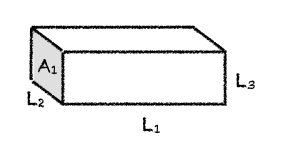
\includegraphics[width=8cm]{fig/Fig1}
\caption{\label{fig:fig1} Bloco retangular.}
\vspace{-0.4cm}
\end{center}
\end{figure}
\begin{num}
\item Determine a área A1 com a incerteza correspondente.
\item Determine o volume desta peça com a incerteza correspondente.
\item Se a precisão necessária para o resultado da área é de 0,5\% podemos considerar este resultado satisfatório?
\end{num}

\item Para determinar a altura de uma cachoeira, algumas pessoas mediram o tempo de queda de pedrinhas que eram soltas, em queda livre, de um mesmo local. Conhecendo o tempo de queda $t$, pode-se calcular a altura $h$ a partir da relação cinemática $h = 1/2 g t^2$ em que $g$ é a aceleração da gravidade. Foi utilizado um cronômetro com precisão de centésimos de segundo e os valores $t_i$ obtidos em 8 medidas estão na seguinte tabela:

\begin{center}
  \begin{tabular}{|>{ \centering\arraybackslash}m{1cm}  |>{ \centering\arraybackslash}m{2cm} |}  \hline
    	& t(s)	 \\ \hline	 	
  1	& 1,30\\ \hline	 
2	&1,09\\ \hline	 
3	&1,03\\ \hline	 
4	&1,27\\ \hline	 
5	&1,18\\ \hline	 
6	&1,31\\ \hline	 
7	&1,24\\ \hline	 
8	&1,15\\ \hline	 
  \end{tabular}
  \end{center}

Considerando $g = (9,784 \pm 0,001)$~m/s$^2$, calcule a altura da cachoeira e a sua incerteza.

\end{num}

%\input{EE3}
%\input{EE4}

\part{Apêndices}
\appendix 
\chapter{Caderno de laboratório}

\vspace{-0.7cm}

\begin{enumerate}
\item {\bf É um documento.} Nele se tem todos os registros cronológicos de um experimentos ou ideia. Portanto, deve ter datas, sem rasuras nem espaços em branco, sem inserções e se possível assinado por quem realizou as anotações.

\item {\bf É pessoal}. Pode haver outros cadernos de uso compartilhado, por exemplo, para equipamentos ou instrumentos de laboratório, etc., onde se registram informações de uso geral, como mudanças introduzidas em configurações experimentais ou estado de conservação dos equipamentos. Mas o caderno de laboratório contem ideias, propostas e modo de colocar a informação que são pessoais, próprias de cada pessoa.

\item {\bf É um registro de anotação em sequência.} Não se devem intercalar resultados nem se corrigir o que está escrito. Em caso de se detectar um erro, se anota na margem o erro encontrado e a página na qual se corrige. Isto permite saber se o erro pode-se voltar a encontrar e a partir de que dados foi corrigido. Por este mesmo motivo não se deve escrever a lápis.

\item {As páginas devem ser numeradas.} Isto permite fazer referência de forma fácil e organizada às anotações anteriores, assim como também indicar na margem onde se corrigem os erros.

\item {As fórmulas e figuras devem ter uma numeração consistente e interna.} Um exemplo prático é numerar todas as fórmulas dentro de cada página ou folha e citá-las por página–fórmula. É importante numerar todas as fórmulas, pois não sabemos no futuro qual necessitaremos citar ou utilizar.

\item {Referências completas.} No caso em que se deva utilizar uma referência externa (roteiro do experimento, artigo, livro, etc.), esta referência deve ser completa. Se uma referência é citada com frequência pode-se utilizar a última página do caderno para registrá-la e citá-la por seu número. Quando citamos alguma coisa, sempre acreditamos que vamos nos lembrar de onde saiu, mas isto só é assim a curto prazo.

\item {\bf Deve-se escrever todos os resultados.} Indicar sempre a maior quantidade de in\-for\-ma\-ção possível do experimento. Todas as condições experimentais devem ser corretamente registradas e deve-se utilizar diagramas claros das configurações experimentais e indicando também cada vez que há uma mudança. Um dado ou informação que hoje parece irrelevante em função do nosso modelo da realidade, pode resultar vital ao descobrir que nossas ideias estavam erradas ou eram incompletas. A falta de um dado de aparência menor pode invalidar tudo o que foi  realizado.

\item {\bf Deve-se escrever o plano.} O que é que se pretende medir, o que é que se procura e as considerações ou razões pelas quais se faz o experimento. O planejamento do experimento e as ideias a serem realizadas devem ser explícitas. A anotação sequencial permite seguir a evolução das idéias, dado vital também para interpretar os resultados, pois os preconceitos condicionam o que se mede e como se mede. Saber o que se pensava no momento de medir vai nos indicar se nesse momento tivemos uma determinada precaução que depois demostrou ser fundamental.

\item {\bf Deve-se escrever as conclusões.} O mesmo vale para o planejamento do experimento.

\item {\bf Fazer uma reorganização periódica das ideias.} Se uma ideia tem evoluído desde o inicio do experimento, é conveniente periodicamente fazer um quadro da situação, passando a limpo o que foi feito, para não ter que reconstruir a história a cada vez.

\end{enumerate}
\chapter{Como escrever um relatório?}
\label{sec:relatorios}
\vspace{-0.7cm}

A idéia desta nota é dar aos alunos de Física Experimental I algumas dicas e re\-co\-men\-da\-ções de como escrever um relatório. Infelizmente, não existe uma “receita” para isto, pois há várias maneiras de fazer um relatório, dependendo do tipo de trabalho realizado e de quem o escreva. Portanto, a organização do relatório pode ser diferente apresentando diferentes distribuições de seções. Nesta nota propõe-se uma estrutura básica com algumas sugestões, mas será com a experiência, com a prática e com as sucessivas correções do professor que os alunos aprenderão a fazê-lo. Escrever um relatório é um aprendizado que se obtém aos poucos.
 
O ponto principal a ser tido em conta é que no relatório deve-se apresentar os resultados obtidos de forma clara e concisa. Para isto, deve-se expor cuidadosamente quais são os objetivos do trabalho realizado, os conceitos físicos básicos necessários para a realização do experimento e como ele foi realizado, entre outros. O relatório tem que ser escrito de modo que um leitor que nunca tenha realizado o experimento descrito, ou a pesquisa realizada, seja capaz de entender e até reproduzir o trabalho a partir do conhecimento adquirido na sua leitura. Para começar, sugere-se a seguinte distribuição:

\begin{itemize}
\item {\bf Título e autores:}  O título deve descrever claramente o conteúdo do trabalho. O relatório tem que ter o(s) nome(s) do(s) autor(es) e as informações relevantes referentes a ele(s). 

\item {\bf Resumo:} Deve dar uma visão completa do trabalho realizado. De forma breve, deve-se descrever qual é o objetivo do mesmo, o que foi feito e qual foi o resultado obtido. 

\item {\bf Introdução:} 
Nela expõem-se as motivações do trabalho e os objetivos a serem atingidos. Deve-se apresentar uma revisão da informação existente sobre o tema em questão. Também, deve-se incluir uma explicação teórica mínima (não copiada de livro, mas elaborada pelos alunos) que permita a compreensão do trabalho e como esta informação está aplicada ao experimento específico. 

\item {\bf Método experimental ou Descrição do experimento:} 
Deve-se descrever em detalhe a configuração experimental utilizada, os métodos utilizados para a realização das medições, incluindo a fundamentação física. Deve-se realizar uma descrição dos aspectos relevantes dos dispositivos e equipamentos utilizados, especificando suas características importantes (precisão dos instrumentos, intervalos de medição, etc). Pode-se representar esquematicamente o dispositivo empregado para a realização do experimento de forma a acompanhar as explicações e facilitar a compreensão do leitor. 

\item {\bf Resultados e discussão: }
Esta seção tem que ser uma continuação natural da In\-tro\-du\-ção e do Método experimental ou Descrição do experimento. Deve-se incluir tabelas dos dados colhidos junto com as suas incertezas e a explicação de como foram avaliadas essas incertezas. Também deve ser realizada uma descrição de como a análise de dados foi realizada e como os resultados foram obtidos. Deve-se incluir também gráficos, junto com as curvas de ajuste dos dados realizados.  Além da análise dos dados, é fundamental realizar uma discussão dos mesmos: sua validade, precisão e a sua interpretação. Dependendo do caso, pode-se realizar uma proposição de um modelo para a descrição dos resultados ou realizar uma comparação com o modelo teórico já discutido na introdução. Caso seja necessária a utilização de equações, elas devem estar explicitadas ou, se já foram introduzidas anteriormente (na introdução), através de uma referência ao número de equação correspondente. 

Levar em conta que, dependendo do relatório e do trabalho apresentados, pode-se separar esta seção em duas independentes, uma de resultados e outra de discussões. 

Figuras e tabelas: cada figura ou tabela deve estar numerada e deve conter uma legenda ao pé que permita entendê-la. A descrição detalhada da figura deve estar incluída também no texto e referenciada pelo número. Os gráficos são considerados figuras, então deverão ser numerados de forma correlacionada com as mesmas.

\item {\bf Conclusões:} 
Deve conter uma discussão de como a partir dos resultados obtidos mostra-se que as hipóteses e objetivos do trabalho foram satisfeitos ou não. Espera-se que a discussão do trabalho seja feita de forma crítica podendo-se propor melhoras ao trabalho realizado, tanto na metodologia empregada quanto nas propostas para ampliar o objetivo do experimento no futuro.

\item {\bf Referências:} 
Deve-se informar a bibliografia citada durante o desenvolvimento do trabalho. A bibliografia pode estar relacionada ao modelo teórico discutido, a referências de equipamento utilizado, ou a artigos de referência no qual o trabalho foi baseado.

\item {\bf Apêndice:} 
Caso seja necessário, pode-se anexar um ou mais apêndices com in\-for\-ma\-ção complementar que ajude a esclarecer o conteúdo das partes anteriores (cálculos realizados para obter um dado resultado, estimativa de incertezas, etc.), mas que no corpo principal do relatório desviariam a atenção do leitor. No(s) a\-pên\-di\-ce(s) coloca-se geralmente informação adicional necessária, mas não fundamental.

\end{itemize}
\chapter{Paquímetro}\label{paquimetro}

\vspace{-0.5cm}


O paquímetro é um instrumento utilizado para medir dimensões de objetos relativamente pequenos, desde uns poucos centímetros até frações de milímetros, com uma precisão da ordem do centésimo de milímetro. Este instrumento é delicado e deve ser manipulado com cuidado e precaução. 

Ele é formado por uma régua com um esquadro num extremo, sobre a qual se desliza o outro esquadro destinado a indicar o valor medido sobre a escala.  Sobre o esquadro móvel encontra-se o nônio que possui uma segunda escala dedicada a marcar as subdivisões do milímetro. Na Figura~\ref{fig:p1} podemos ver um desenho de um paquímetro típico.

\begin{figure}[h]
\begin{center}
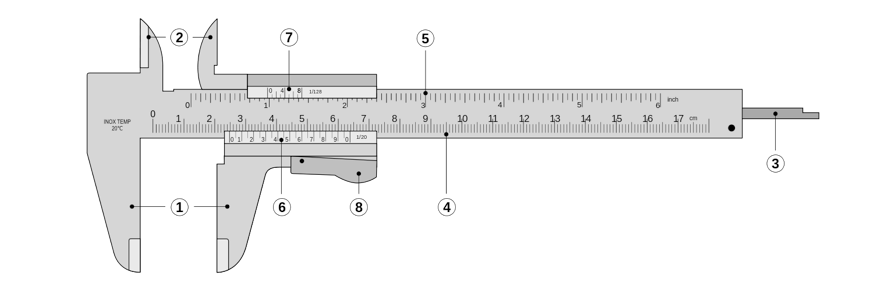
\includegraphics[width=14cm]{fig/Paquimetro1}
\caption{\label{fig:p1} Paquímetro formado por: \textcircled{1} Encostos para medidas externas; \textcircled{2} Orelhas para medidas internas; \textcircled{3} Haste de profundidade; \textcircled{4} Escala principal inferior (graduada em centímetros e milímetros); \textcircled{5} Escala principal superior (graduada em polegadas e frações de polegadas); \textcircled{6} Nônio ou vernier para leitura das frações de milímetros em que esteja dividido; \textcircled{7} Nônio ou vernier para leitura das frações de polegada em que esteja dividido; \textcircled{8} Propulsor e trava.}
\vspace{-0.5cm}
\end{center}
\end{figure}

Para utilizar o paquímetro, primeiramente se separam os encostos para que o objeto a ser medido possa ser colocado entre eles, logo se fecham estes encostos de forma que o objeto fique preso ao mesmo e se bloqueia o movimento do esquadro móvel para poder realizar a leitura do valor medido. Usaremos o exemplo mostrado na Figura~\ref{fig:p2} para facilitar a explicação de como fazer a leitura. 

\begin{figure}[h]
\begin{center}
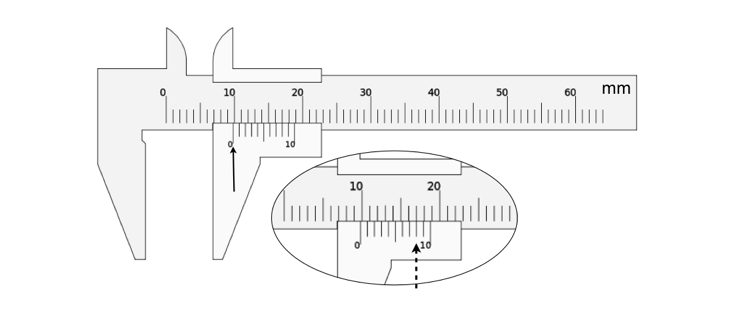
\includegraphics[width=14cm]{fig/Paquimetro2}
\caption{\label{fig:p2} Exemplo de uma medição realizada com paquímetro graduado em mm e com um nônio com 10 divisões. Valor medido (0,98 $\pm$ 0,01) cm. Ver texto.}
\vspace{-0.5cm}
\end{center}
\end{figure}

O primeiro passo é fazer a leitura sobre a escala principal (Figura~\ref{fig:p1}) e para isso observamos a posição do zero do nônio, que no exemplo está levemente deslocada à direita dos 9 mm (seta cheia na figura~\ref{fig:p2}). Desta forma temos a primeira parte da medida, sendo 0,9 cm. Vemos que as seguintes marcas do nônio também estão levemente deslocadas à direita e que esta diferença vai se reduzindo paulatinamente. Verificamos que a oitava marcação sobre o nônio coincide com a marcação com a régua principal (seta tracejada na Figura~\ref{fig:p2}) e logo as marcas do nônio vão ficando progressivamente à esquerda das marcas da régua fixa. Portanto a segunda parte da leitura nos diz que o valor medido é de 0,98 cm com uma incerteza de 0,01 cm.  Para a determinação da incerteza, considerada aqui como a mínima divisão do instrumento, temos que determinar o número de subdivisões do milímetro dado pelo nônio.  No caso do exemplo, temos 10 subdivisões, sendo a incerteza 1 mm dividido 10, ou seja 0,1 mm.  Finalmente o resultado da medição é: (0,98 $\pm$ 0,01) cm.

\underline {Importante:} Lembrar de verificar que o paquímetro esteja corretamente calibrado, ou seja que quando não haja abertura dos dois encostos, o zero da escala principal e do nônio sejam coincidentes.  

Mais informações sobre o uso do paquímetro podem ser encontradas na página  \url{http://www.stefanelli.eng.br/webpage/metrologia/p-nonio-milimetro-05.html}.
\chapter{Trilho de Ar}\label{trilho}
\vspace{-0.3cm}
O trilho de ar é um sistema que permite estudar movimentos unidimensionais reduzindo drasticamente as forças de atrito habitualmente presentes. Ele é composto de chapas metálicas de perfil reto, com pequenos orifícios regularmente espaçados nas faces  laterais.  

Injeta-se ar comprimido dentro do trilho que sai através dos orifícios gerando desta forma um colchão de ar entre o trilho e o carrinho de cerca de 0,5 mm de espessura. Este colchão de ar faz com que o carrinho "flutue", provocando assim uma grande redução do atrito.  O atrito residual é devido principalmente à fricção com o ar. Nas extremidades do trilho sempre deve-se colocar os pára-choques formado por um suporte com elásticos. 

O sistema trilho de ar e carrinho devem ser cuidadosamente tratados para evitar que eles se sofram deformações ou marcas que comprometam a redução do atrito.  Para isto devemos evitar choques mecânicos fortes, tanto ente o carrinho e o trilho como entre dois carrinhos. Evitar quedas dos carrinhos, mesmo que sejam de uns poucos centímetros, manuseando-os com segurança e muito cuidado. Em continuação enumeramos alguns cuidados extras na hora de utilizar o sistema trilho-carrinho, a saber:
\vspace{-0.3cm}
\begin{iten}

\item Nunca movimente os carrinhos sobre o trilho quando não houver ar saindo pelos orifícios do trilho ou se o ar que sai é muito fraco (neste caso deve se aumentar a potência do ar comprimido), pois serão produzidos arranhões.

\item Quando se colocar massas em cima dos carros, é fundamental que estas sejam distribuídas simetricamente para evitar desbalanceamentos do carrinho quando flutua podendo encostar certas partes dele no trilho.  Desta forma não só poderão ser produzidos arranhões no trilho senão como a hipóteses de atrito desprezível não será verificada. 

\item O trilho é apoiado sobre pequenas hastes numa base em perfil de alumínio. Estas hastes têm como função permitir o nivelamento do trilho. Com o tempo e o uso constante, o trilho de ar tende a se deformar criando "barrigas".  A consequência principal destas barrigas é os carrinhos passam a ter um movimento irregular. O nivelamento do trilho é uma operação trabalhosa e delicada, por isso deve-se estar seguro da necessidade de nivelamento antes de começar a mexer.

\end{iten}
\chapter{Sistema de Video}\label{image}

\vspace{-0.5cm}

\section*{Configuração Câmera}

Para a realização dos filmes os passos a seguir são:

\begin{enumerate}
\item Ligue a câmera e verifique que o cartão de memória esteja vazio. %Para isto tem que ir ao menu e escolher com o cursor a terceira opção como é mostrado na Figura~\ref{fig:camera}-A. Uma vez no menu com o cursor da esquerda escolha a opção ``Apagar", dê ``OK" quantas vezes seja necessário para apagar as fotos e filmes do cartão de memória.

\item Configure a câmera para a realização do filme. 
\begin{itemize}
\item Para a câmera Olympus: %Entre no menu e escolha a segunda opção como indicado na Figura~\ref{fig:camera}-B.  A configuração escolhida deve ser: 
\begin{enumerate}
\item {\bf Tamanho De Imag} VGA
\item {\bf Imagens Por Seg.} 15 ou 30 fas (fotos por segundo) 
\item {\bf Microfone} Desl.  (desligado)
\item {\bf Modo AF}: configure a câmera para que sempre faça foco no objeto de interesse, mesmo quando ele esteja em movimento. Novamente, entre no menu e escolha a primeira opção como indicado na Figura~\ref{fig:camera}-C. No menu da esquerda escolha a terceira opção ``Modo AF" e logo ``Rastreia AF". Dê ``OK"  e pressione o botão do menu para sair do mesmo.
\end{enumerate}

\item Para a câmera Nikon Coolpix s3600, aperte o botão ``Menu", selecione o ícone de câmera de vídeo conforme a Figura~\ref{fig:nikon} e selecione:
\begin{enumerate}
\item {\bf Opções de vídeo}: 480/30p
\item {\bf Modo foco automático:} AF-F AF constante
\item {\bf VR do vídeo}: desligado
\end{enumerate}
\item Para a câmera Sony Cyber-shot, aperte o botão ``Menu" e busque as opções a seguir, conforme a Figura~\ref{fig:sony}: 
\begin{enumerate}
\item {\bf Tamanho Filme:} VGA
\item {\bf ACT:} STD movimentação moderada (nem todas as câmeras tem essa opção no menu à esquerda, com um ícone de mão)
\end{enumerate}
\end{itemize} 
\end{enumerate}

Desta forma sua câmera está configurada e você pode começar a fazer sua aquisição de dados. 
\begin{figure}[t!]
\begin{center}
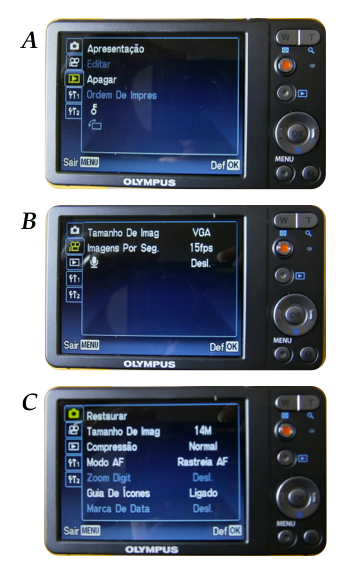
\includegraphics[width=9cm]{fig/CameraOlympus.png}
\caption{\label{fig:camera} Configuração da câmera Olympus.}
\vspace{-0.5cm}
\end{center}
\end{figure}

\begin{figure}[h!]
\begin{center}
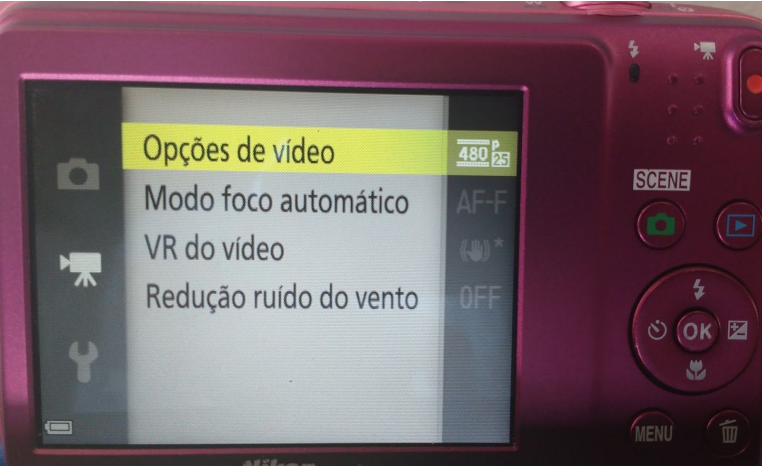
\includegraphics[width=9cm]{fig/cameraNikon.png}
\caption{\label{fig:nikon} Configuração da câmera Nikon.}
\vspace{-0.5cm}
\end{center}
\end{figure}

\begin{figure}[h!]
\begin{center}
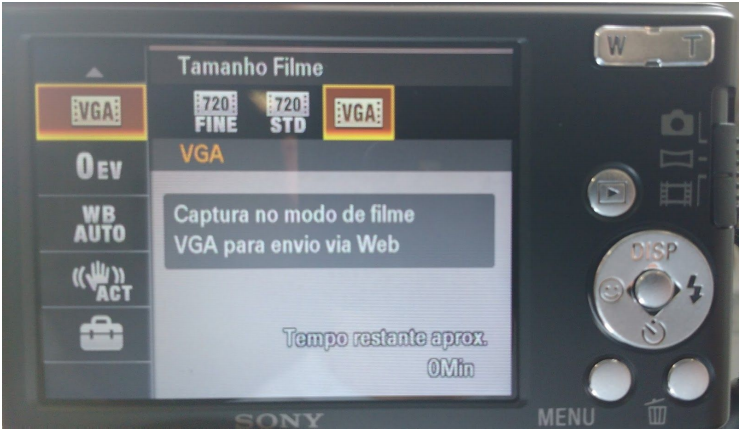
\includegraphics[width=9cm]{fig/cameraSony.png}
\caption{\label{fig:sony} Configuração da câmera Sony.}
\vspace{-0.5cm}
\end{center}
\end{figure}
\newpage
\section*{Leitura manual da posição do carrinho}
\begin{enumerate}

\item Uma vez registrado o movimento do carrinho com a câmera proceda a baixar o filme que você fez numa pasta no desktop do seu computador chamada MRU. Para algumas câmeras, o video é salvo no formato MP4 e precisa ser convertido em AVI para análise no programa ImageJ. Um tutorial para conversão dos videos encontra-se nas bancadas, próximo ao computador.
\item Abra o programa ImageJ.
\item No ImageJ abra o filme que você fez em formato AVI. Aparecerá uma tela com algumas indicações como se mostra na Figura~\ref{fig:frame}, “First Frame 1”, “Last Frame 135”, que podem em princípio ser alteradas pelo usuário. Essas informações correspondem ao número de imagens contidas no filme e permitem que escolhamos apenas algumas delas para serem exibidas. Mantenha como está e tecle “Ok”.
\begin{figure}[t!]
\begin{center}
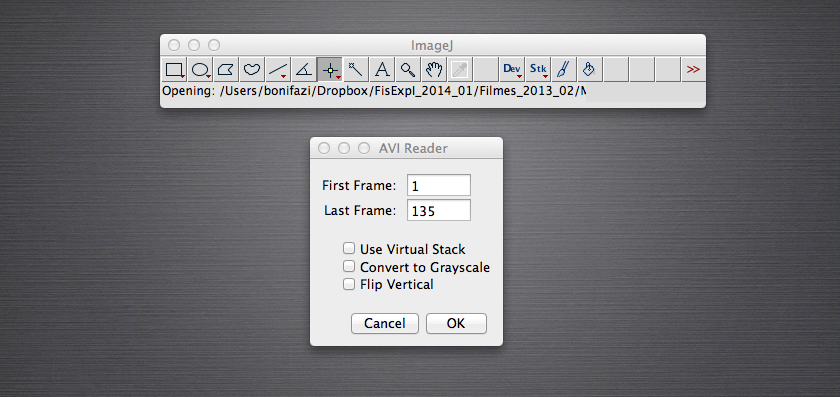
\includegraphics[width=11cm]{fig/frame}
\caption{\label{fig:frame} ImageJ: tela de inicio para carregar o filme.}
%\vspace{-0.5cm}
%\end{center}
%\end{figure}
%\begin{figure}[h]
%\begin{center}
\vspace{0.3cm}
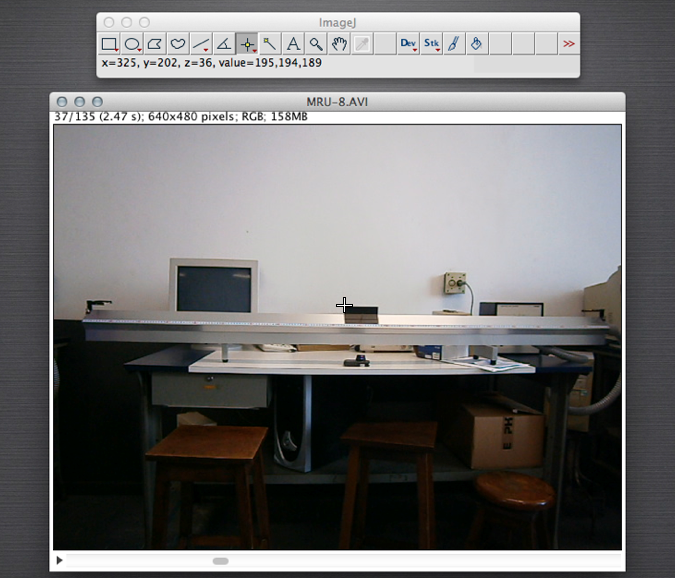
\includegraphics[width=11cm]{fig/cursor}
\caption{\label{fig:exMovie} ImageJ: posição do cursor sobre a imagem.}
\vspace{-0.6cm}
\end{center}
\end{figure}

\item Após o filme aberto você pode escolher a ferramenta de “zoom” que fica na barra de ferramentas do programa para ver melhor as imagens. A resolução das imagens não é muito boa, mas não precisamos mais do que isso para fazer a análise do experimento.
\item Experimente passar o cursor do mouse sobre a imagem. Você verá que embaixo da barra de ferramentas do ImageJ aparecerão alguns números, por exemplo, na Figura~\ref{fig:exMovie}: x=325, y=202, z=36, value = 195. As letras “x” e “y” correspondem à posição do cursor em “pixels” no sistema de referência mostrado na Figura~\ref{fig:exMovie}. A letra “z” corresponde à ordem em que imagem foi capturada em relação ao início do filme. Finalmente, “value” corresponde aos níveis de vermelho, verde e azul da imagem, nesta ordem. Para as análises que faremos, só utilizaremos a posição “x e y” do cursor.
\item Observe agora no canto superior esquerdo das imagens do filme (Figura~\ref{fig:exMovie}). Aparecem números semelhantes a “37/135 (2.47s); 640x480 pixels; RGB; 158 MB”. O primeiro deles significa que está sendo exibida a imagem 37 de um total de 135. O instante de tempo no qual essa imagem foi capturada em relação ao início do filme é indicado pelo número entre parênteses “2.47s” que é dado por $1/15 \times 37$~s (onde 1/15 corresponde a 15 fotos ou {\it frames}  por segundo), “640 X 480 pixels” corresponde às dimensões da imagem em número de “pixels”, “RGB” corresponde à qualidade da imagem, e “158 MB” corresponde ao espaço de memória do computador que foi utilizado para guardar o filme. Para nossas análises o número importante dentre esses é o que corresponde ao número de imagem e ao instante de tempo em que a imagem foi capturada. \underline{Observação}: estes números serão diferentes para cada filme.
\end{enumerate}


\section*{Rotação do Filme}

Para realizar a análise dos dados, é necessário que a medida do deslocamento do carrinho seja apenas em uma dimensão, por exemplo, na horizontal.  Se o eixo horizontal da câmera não está bem alinhado com o trilho, precisamos realizar uma rotação do filme antes de proceder à leitura da posição do carrinho. Portanto, o primeiro passo é a determinação do ângulo de rotação.  A mesma pode ser realizada de duas formas diferentes:

\vspace{-0.7cm}
\subsection*{\underline{Forma manual}}
\vspace{-0.2cm}
\begin{enumerate}
\item Determine com os cursores as coordenadas ``x e y" das extremidades do trilho, tendo desta forma $(x_1,y_1) e (x_2, y_2)$ como se mostra na figura~\ref{fig:coord}.
\item Utilizando trigonometria, e utilizando uma calculadora, determine o ângulo de inclinação como o $\arctan{(y_2-y_1)/(x_2-x_1)}$. \underline{Observação:} o ângulo tem que ser determinado em graus.
\end{enumerate}

\vspace{-0.9cm}
\subsection*{\underline{Forma automática}}
\vspace{-0.2cm}
\begin{enumerate}
\item Escolha o botão de “\^Angulo” (círculo na Figura~\ref{fig:angulo}-A), que fica na barra de ferramentas do programa ImageJ para poder marcar o ângulo que quer ser determinado. 
\item Movimente o cursor para marcar os três pontos que vão determinar o ângulo que o trilho forma com a horizontal (linhas cheias sobre o filme na Figura~\ref{fig:angulo}-B). Faça click cada vez que esteja na posição desejada.
\item Escolha a opção "Analyze" do menu principal e "Measure" do sub-menu.
\item O resultado será mostrado em uma outra janela (Figura~\ref{fig:angRes}), entre os quais estará o valor do ângulo desejado em graus.

\begin{figure}[t!]
\begin{center}
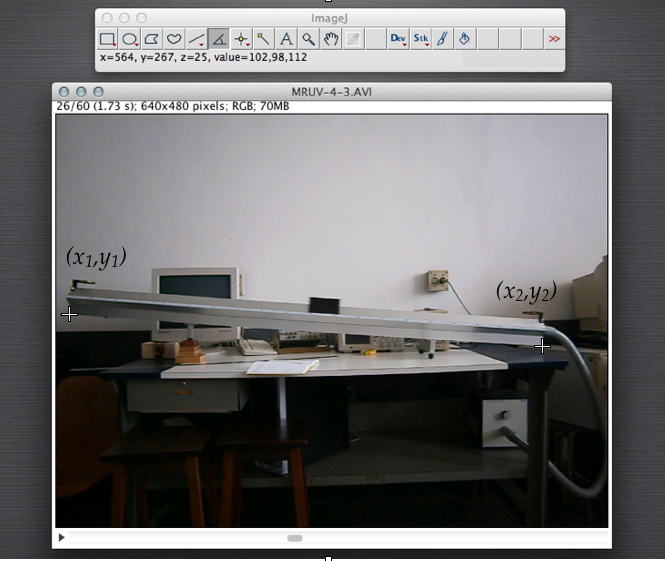
\includegraphics[width=9cm]{fig/coordman}
\caption{\label{fig:coord} ImageJ: determinação das coordenadas $(x_1,y_1) e (x_2, y_2)$, ver texto.}
\vspace{0.5cm}
%\end{center}
%\end{figure}
%\begin{figure}[h]
%\begin{center}
%\vspace{-0.3cm}
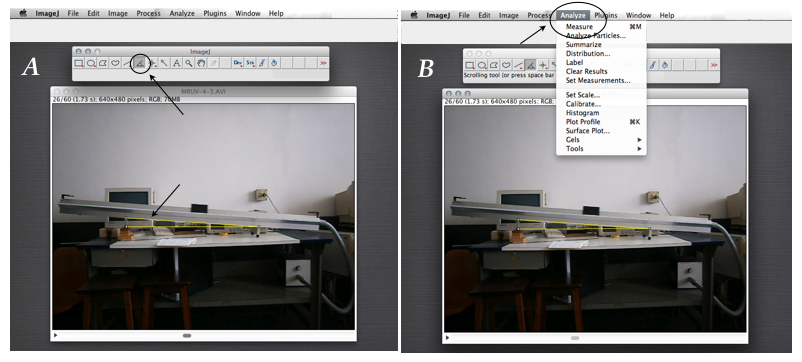
\includegraphics[width=16cm]{fig/AnguloAuto}
\caption{\label{fig:angulo} ImageJ: determinação do ângulo de inclinação do trilho, ver texto.}
\vspace{-0.5cm}
\end{center}
\end{figure}

Uma vez determinado o ângulo, devemos proceder a realizar a rotação do Filme. Para isto, deve seguir os seguintes passos: 
\begin{enumerate}
\item Escolha a opção ``Imagem" do menu principal, logo ``Transform" e finalmente ``Rotate", como mostrado na Figura~\ref{fig:rotate}-A.
\item Uma nova janela será aberta onde deve-ser informado o valor do ângulo de rotação, no nosso exemplo, o mesmo é de 4,101 graus (Figura~\ref{fig:angRes}). Este ângulo deve ser informado com o sinal negativo ($-$) se queremos realizar uma rotação no sentido anti-horário ou com sinal positivo ($+$) se a rotação é no sentido horário.
\item {\bf Como a rotação é uma ação definitiva} e não pode ser refeita, utilizar sempre o ``Preview" para poder ter certeza de que se está realizando a rotação desejada (ver Figura~\ref{fig:rotate}-B) antes de dar o ``OK" final.
\end{enumerate}

\begin{figure}[h!]
\begin{center}
\vspace{0.3cm}
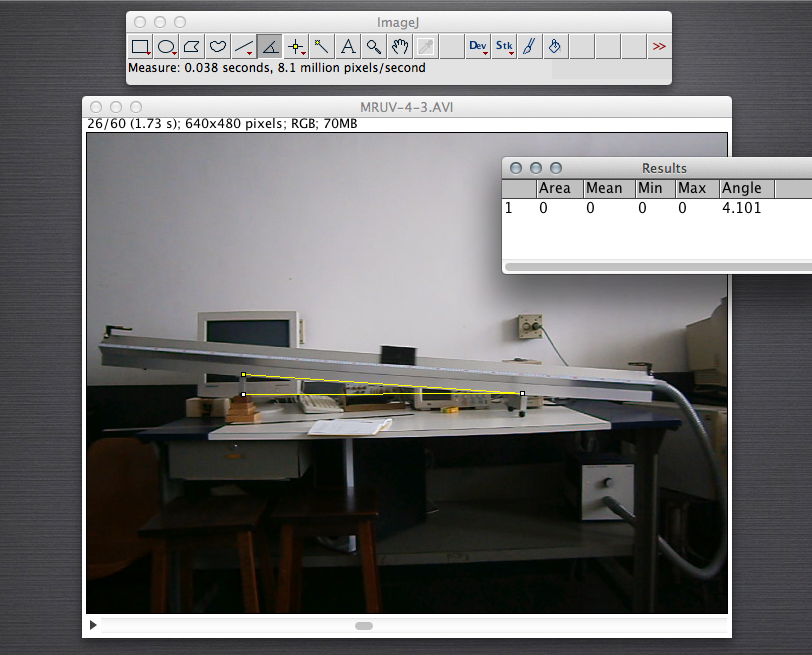
\includegraphics[width=10cm]{fig/AnguloResultado}
\caption{\label{fig:angRes} ImageJ: valor do ângulo de inclinação do trilho}
\vspace{0.5cm}
%\end{center}
%\end{figure}
%\begin{figure}[h]
%\begin{center}
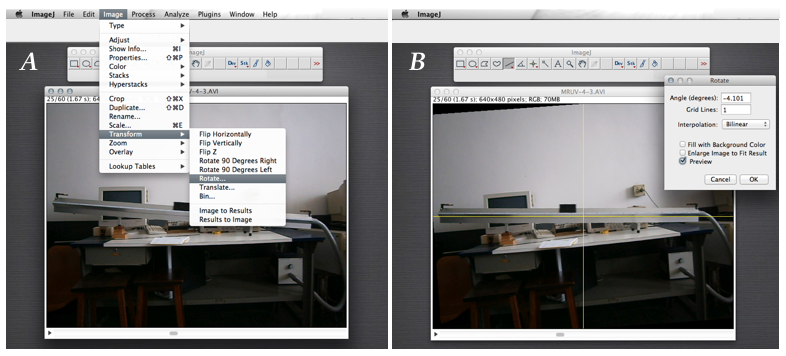
\includegraphics[width=16cm]{fig/Rotate}
\caption{\label{fig:rotate} ImageJ: rotação do filme por um determinado ângulo, ver texto}
\vspace{-0.5cm}
\end{center}
\end{figure}
\end{enumerate}


\chapter{Programa QtiPlot}\label{QtiPlot}

\vspace{-0.7cm}

Ao longo do curso vamos realizar gráficos e ajustes lineares (ajustes por uma reta), para isto vamos aprender a utilizar um programa chamado de QtiPlot.  Este programa pode ser baixado gratuitamente da internet, ou da página pessoal do Prof. Angelo Gomes em: 
\url{http://www.if.ufrj.br/~amgomes/qtiplotinfo.html}. 

Para descompactar o mesmo você deverá fornecer uma senha, a mesma é: fisexp2-2009

O Prof. Angelo Gomes preparou um tutorial que ajuda a aprender a utilizar o QtiPlot. Para acessar ao mesmo, basta com ir para \\
\url{http://www.if.ufrj.br/~amgomes/tutorialqtiplot-pag1.html}

Qualquer dúvida ou problema, entrar em contato com seu professor e/ou monitor.



\end{document}

%%%%%%%%%%%%%%%%%%%%%%%%%%%%%%
